
\section{Probabilidad Condicional}

La probabilidad condicional nos provee una forma de razonar acerca de la salida
o resultado de un experimento, basado en información parcial. Algunos ejemplos
de estos experimentos podrían ser los siguientes:

\begin{itemize}
\item En un experimento en el cual tiramos dos dados sucesivamente, te dicen que
la suma de los dados es 9. ¿Qué tan probable es que el primer dado haya caído 6?

\item En un juego de adivinanzas de palabras, la primera letra de la palabra es
\textit{t}. ¿Cuál es la probabilidad de que la siguiente palabra sea \textit{h}?

\item ¿Qué  tan probable es que una persona tenga cierta enfermedad dado que su
examen médico dió negativo?
\end{itemize}

En términos más precisos, dado un experimento, un espacio de muestreo y una ley
de probabilidad, suponiendo que sabemos que la salida está dentro de un evento
dado $B$. Deseamos cuantificar la probabilidad de que la salida pertenece a
algún otro evento $A$. Así, podemos construir una nueva probabilidad que tome en
cuenta el conocimiento disponible: una ley de probabilidad para cuaquier evento
$A$. Especificamente, la probabilidad condicional de $A$ dado $B$, denotado por
$P(A|B)$ \cite{vsirca2016probability}.

Para calcular $P(A|B)$ consideramos aquellos resultados del evento $A$ que están en
el evento $B$. Esto nos da los resultados en el evento $A \cap B$ y nos lleva al
teorema de la probabilidad condicional.

\begin{theorem}{Probabilidad Condicional}{conditional_probability}
Sea $S$ el espacio de muestro para un experimento $E$ y $A$, $B \subseteq S$,
entonces la probabilidad condicional de $A$ dado $B$ está dada por:
    \begin{equation}
        P(A|B) = \frac{P(A \cap B)}{P(B)}
        \label{eq:conditionalProbability}
    \end{equation}

Siempre que $P(B)>0$.

Particularmente, todas las propiedades de las leyes de la probabilidad
permanecen válidas para las leyes de la probabilidad condicional.

\begin{itemize}
    \item La probabilidad condicional puede verse también como una ley de
    probabilidad en un nuevo universo $B$, ya que toda la probabilidad condicional
    está concentrada en $B$.

    \item Si todos los resultados son finitos e igualmente probables, entonces:
        \begin{equation}
            P(A|B)=\frac{\text{número de elementos de }A \cap B}{\text{número de elementos de }B}
        \end{equation}
\end{itemize}
\end{theorem}


\def\firstcircle{(0,0) circle (1.5cm)}
\def\secondcircle{(0:2cm) circle (1.5cm)}
\def\rectangle{(-2,-2) rectangle (4,2)}

\colorlet{circle edge}{black!50}
\colorlet{circle area}{gray!20}

\tikzset{filled/.style={fill=circle area, draw=circle edge, thick},
    outline/.style={draw=circle edge, thick}}

\setlength{\parskip}{5mm}

\begin{figure}[h]
    \centering
    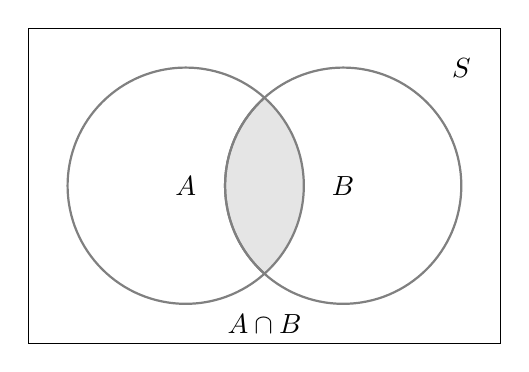
\begin{tikzpicture}
        \draw \rectangle;
        \begin{scope}
            \clip \firstcircle;
            \fill[filled] \secondcircle;
        \end{scope}
        \draw[outline] \firstcircle node {$A$};
        \draw[outline] \secondcircle node {$B$};
        \node[anchor=south] at (current bounding box.south) {$A \cap B$};
        \node at (3.5,1.5){$\mathbb S$};
    \end{tikzpicture}
    \caption{Representación del concepto intuitivo de la probabilidad condicional.}
    \label{fig:coditionalProbability}
\end{figure}

\begin{figure}[h]
    \centering
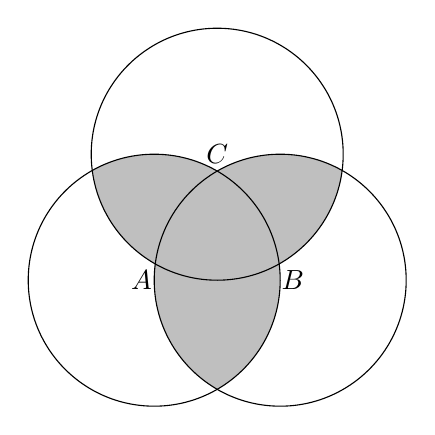
\begin{tikzpicture}[scale = 0.8]
    \begin{scope}
    %\clip (-1,0) circle (2);
    \clip (1,0) circle (2);
    \clip (0,2) circle (2);
    \fill[gray!50] (0,0) circle (5);
    \end{scope}
    \begin{scope}
    \clip (-1,0) circle (2);
    %\clip (1,0) circle (2);
    \clip (0,2) circle (2);
    \fill[gray!50] (0,0) circle (3);
    \end{scope}
    \begin{scope}
    \clip (-1,0) circle (2);
    \clip (1,0) circle (2);
    %\clip (0,2) circle (2);
    \fill[gray!50] (0,0) circle (3);
    \end{scope}
    \draw (-1,0) circle (2);
    \node at (-1.2,0){$A$};
    \draw (1,0) circle (2);
    \node at (1.2,0){$B$};
    \draw (0,2) circle (2);
    \node at (0,2){$C$};
\end{tikzpicture}
\caption{Representación de la unión de las intersecciones de tres conjuntos diferentes.}
\label{fig:unionIntersection}
\end{figure}


\textbf{Observaciones y consideraciones de la probabilidad condicional:}

\begin{itemize}
\item La probabilidad $P(A|B)$ es una actualización de $P(A)$, basada en el
conocimiento de que ocurrió el evento $B$.

\item De la Ec.(\ref{eq:conditionalProbability}), tanto $P(A \cap B)$ como
$P(A)$ se calculan a partir del espacio muestral original.

\item Las probabilidades tienen sutiles cambios dependiendo de la información
exacta de la condición implicada en el evento A.
\end{itemize}

\subsection{Propiedades de las leyes de la probabilidad}

Las leyes de la probabilidad tienen propiedades que pueden deducirse de los
axiomas \cite{walpole2012probabilidad}. Algunas de ellas, son las que se muestran
a continuación.

\begin{tcolorbox}[colback=gray!5!white,colframe=gray!60!black,title=Resumen: Propiedades de las leyes de la probabilidad]
    Sean $A$, $B$ y $C$ eventos:

    \begin{itemize}
        \item
        \begin{equation}
            \text{Si } A \subset B, \text{entonces } P(A) \leq P(B)
            \label{eq:propProb1}
        \end{equation}
        
        \item 
        \begin{equation}
        P(A \cup B) = P(A) + P(B) - P(A \cap B)
        \label{eq:propProb2}
        \end{equation}

        \item 
        \begin{equation}
            P(A \cup B) \leq P(A) + P(B)
            \label{eq:propProb3}
        \end{equation}

    \item
    $P(A \cup B \cup C)=$
    \begin{equation}
        P(A) + P(B) + P(C) - P(A \cap B) - P(A \cap C) - 
        P(B \cap C) + P(A \cap B \cap C)
        \label{eq:propProb4}
    \end{equation}
    \end{itemize}
\end{tcolorbox}

De la Ec.(\ref{eq:conditionalProbability}) podemos hacer que:

\begin{center}
$P(B \cap A) = P(A \cap B) = P(A) \  P(B|A)$, 
\end{center}

y cambiando los roles de $A$ y de $B$, tenemos que:

\begin{center}
    $P(A \cap B) = P(B \cap A) = P(B) \ P(A|B)$, 
\end{center}

esto resulta en:

\begin{center}
    $P(A)P(B|A) = P(A \cap B) = P(B) \ P(A|B)$,
\end{center}

que comunmente llamamos \textit{regla de la multiplicación}.

Para verificar algunas de las propiedades de las leyes de la probabilidad,
podemos usar diagramas de Venn, Fig. (\ref{fig:unionIntersection}). Si $A \subset
B$, entonces $B$ es la unión de eventos los eventos disjuntos $A$ y $A_c \cap
B$, por lo que por el axioma de adición, tenemos:

\begin{center}
    $P(B) = P(A) + P(A^c \cap B) \geq P(A)$.
\end{center}

Como observamos en la Fig. (\ref{fig:difer}), podemos expresar los eventos $A
\cup B$ y $B$ como unión de conjuntos disjuntos:

\begin{center}
    $A \cup B = A \cup (A^c \cap B)$,
\end{center}

\begin{center}
    $B = (A \cap B) \cap (A^c \cap B)$
\end{center}

Usando el axioma de adición, tenemos:

\begin{center}
    $P(A \cup B) = P(A) + P(A^c \cap B)$,
\end{center}

\begin{center}
    $P(B) = P(A \cap B) + P(A^c \cap B)$
\end{center}

Si despejamos $P(A^c \cap B)$ de la seguda igualdad y la sustituimos en la
primera, tenemos:

\begin{center}
    $P(A \cup B) = P(A) + P(B) - P(A \cap B)$,
\end{center}

con lo que podemos verificar la Ec. \eqref{eq:propProb3}

\begin{figure}
% Set B but not A
\centering
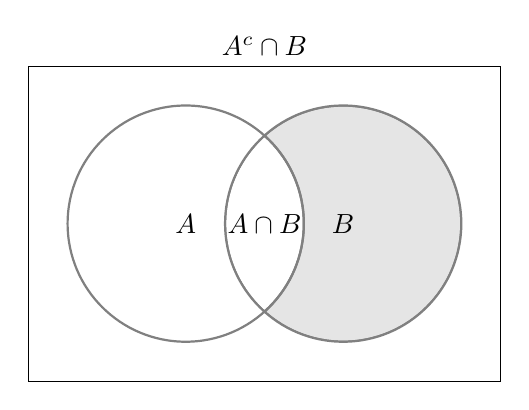
\begin{tikzpicture}
    \draw \rectangle;
    \begin{scope}
        \clip \secondcircle;
        \draw[filled, even odd rule] \firstcircle
                                     \secondcircle node {$B$};
    \end{scope}
    \draw[outline] \firstcircle node {$A$}
                   \secondcircle;
    \node[anchor=south] at (current bounding box.north) {$A^c \cap B$};
    \node at (1,0){$A \cap B$};
\end{tikzpicture}
\caption{Representación gráfica de los eventos $A \cup B$, como unión de eventos disjuntos.}
\label{fig:difer}
\end{figure}

\subsection{Teorema de la probabilidad total}
\begin{theorem}{Teorema de la probabilidad total}{TotalProbabilityTheorem}
Sean $A_1, ..., A_n$ eventos disjuntos que forman una partición de un espacio
muestral, y asumiendo $P(A_i)>0$, para todo $i$. Entonces,
para cualquier evento $B$, tenemos:

\begin{center}
    $P(B) = P(A_1 \cap B) + ... + P(A_n \cap B)$
\end{center}

\begin{equation}
    =P(A_1)\ P(B|A_1) + ... + P(A_n) \ P(B|A_n)
\end{equation}

\end{theorem}


\subsection{Teorema de Bayes}

\begin{theorem}{Teorema de Bayes}{BayesTheorem}
Sean $A$ y $B$ dos eventos cuyas probabilidades son diferentes de cero,
entonces:
    \begin{equation}
        P(B|A) = \frac{P(A|B) \ P(B)}{P(A)}
        \label{eq:BayesTheorem}
    \end{equation}

La implicación más importante de la Ec. (\ref{eq:BayesTheorem}) es que permite
encontrar probabilidades condicionadas $P(B|A)$ en términos de $P(A|B)$, cuando
esta última resulta más fácil de calcular directamente.
\end{theorem}
